\documentclass[../main]{subfiles}

\begin{document}
\subsection{Principio de Arquímedes}
El Principio de arquímedes da el siguiente enunciado:\\
\textit{Si un cuerpo está parcial o totalmente sumergido en
un fluido, éste ejerce una fuerza hacia arriba sobre el cuerpo igual al peso del fluido
desplazado por el cuerpo.} \parencite{sears}

\subsection{Empuje $(\vec{E})$}
La fuerza descrita por el Principio de Arquímedes puede ser formulado de la siguiente manera:
\begin{figure}[H]
    \centering
    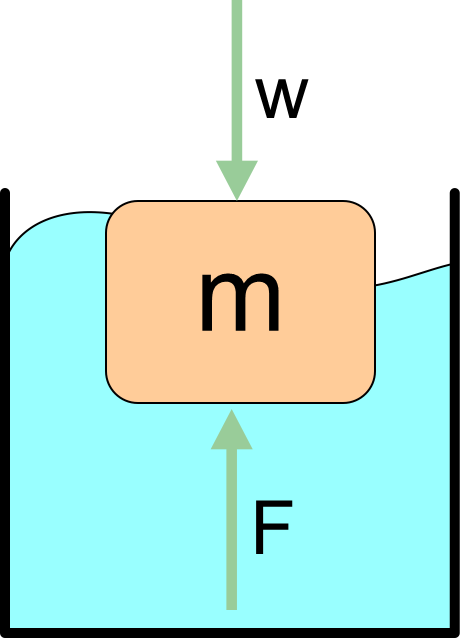
\includegraphics[width=0.2\linewidth]{resources/empuje.png} 
    \caption{Diagrama de cuerpo libre de un cuerpo en equilibrio en un líquido.}
    \label{fig:empuje}
\end{figure}
Del gráfico \ref{fig:empuje} y usando la segunda Ley de Newton:
\begin{align*}
    \vec{F_R} &= m \cdot \vec{a} \\
    \vec{W} + \vec{F} &= m \cdot \vec{a}
\end{align*}
Pero dado que el cuerpo está en equilibrio:
\begin{align}
    \vec{W} + \vec{F} &= 0 \nonumber \\
    \vec{F} &= - \vec{W} \nonumber \\
    \label{force_mass_gravity}
    \vec{F} &= - m \cdot \vec{g}
\end{align}
Teniendo en cuenta el Principio de Arquímedes, entonces:
\begin{equation} \label{mass_density_volume}
     m = \rho \cdot V_{desplazado}
\end{equation}
Reemplazando \ref{mass_density_volume} en \ref{force_mass_gravity}:
\begin{equation*}
    \vec{F} = - \rho \cdot V_{desplazado} \cdot \vec{g}
\end{equation*}
A esta fuerza $\vec{F}$ se la denomina \textit{empuje $(\vec{E})$}
\begin{equation} \label{empuje_eq}
    \Vec{E} = - \rho \cdot V_{desplazado} \cdot \vec{g}
\end{equation}
Donde:
\begin{itemize}
    \item $\rho$: densidad del líquido
    \item $V_{desplazado}$: volumen de líquido desplazado
    \item $\vec{g}$: gravedad
\end{itemize}
\subsection{Torque $(\vec{\tau})$}
Se define como: \parencite{sears}
\begin{equation} \label{torque}
    \vec{\tau}_O = \vec{r} \times \vec{F}
\end{equation}
Donde:
\begin{itemize}
    \item $\vec{\tau}_O$: vector Torque debido a la fuerza
    $\vec{F}$ con respecto al punto O
    \item $\vec{r}$: vector de O a donde actúa $\vec{F}$
    \item $\vec{F}$: fuerza $\vec{F}$
\end{itemize}
El torque mide \textit{que tan efectiva es una fuerza para crear o modificar
un movimiento de rotación}. \parencite{sears}

\subsection{Torque Resultante $(\vec{\tau}^{\,r})$}
Mide el torque total sobre una partícula, se calcula como la
sumatoria de todos los torques que actuan sobre la partícula.
\begin{equation} \label{torque_resultante1}
    \vec{\tau}_O^{\,r} \, = \, \sum^n_{k=1} \vec{\tau}_k
\end{equation}
Además, está presente la siguiente ecuación:
\begin{equation} \label{torque_resultante2}
    \vec{\tau}_O^{\,r} \, = \, I \cdot  \vec{\alpha}
\end{equation}
Donde:
\begin{itemize}
    \item $I$: momento de inercia en el punto O
    \item $\vec{\alpha}$: aceleración angular en el punto O
\end{itemize}

\subsection{Segunda condición de Equilibrio}
Se da cuando el torque resultante es igual 0.
\begin{equation} \label{equilibrio_2}
    \vec{\tau}_O^{\,r} \, = 0
\end{equation}
Interpretando la ecuación \ref{equilibrio_2}, cuando esto ocurre, la aceleración
angular es nula, provocando que no exista movimiento de rotación en el cuerpo.

\subsection{Desviación Estándar}
La desviación estándar es una medida de extensión o
variabilidad en la estadística descriptiva.
Se utiliza para calcular la variación o dispersión
en la que los puntos de datos individuales difieren
de la media.
\begin{equation} \label{desviacion_eq}
    \sigma = \sqrt{\frac{\sum^N_{i=1} (x_i - \overline{x})^2}{N}}
\end{equation}
\end{document}
